\section{Model description}

\subsection{General approach}

%Most models that integrate water resources and agricultural economics are composed of an economic optimization component linked to some type of hydrologic model that provides physical constraints on the amount of water and land available for agricultural production \citep{Harou2009b}.

%Classic linear optimization models of agriculture implemented to simulate agent behavior often produce unrealistic results because it is not possible to explicitly account for all of the variables affecting farmer decisions. To overcome this problem, many modern economic optimization models used in policy analysis are based on a methodology called positive mathematical programming, PMP Howitt \citep{Howitt1995, Howitt2012}. PMP reduces the amount of data and artificial restrictions needed to calibrate classic optimization models. It also avoids overspecialization in crop production and ensures that the model calibrates to observed conditions. 

%Models based on PMP have been used intensively in drought analysis and policy design \citep{Connell-Buck2011, Medellin-Azuara2011, USBoR2011, DWR2009, Maneta2009c, Cobourn2011}, however this method relies on field surveys that can introduce biases in the analysis. If the surveyed farms or the year of the survey are not representative of the group or the long term conditions, the calibration may have a bias toward the conditions observed in the farm the year of the survey. In addition, the PMP methodology is based on the solution of a deterministic nonlinear optimization program. This may provide a false sense of precision in the calibration and simulation outputs because deterministic methods do not reflect modeling errors derived from uncertainties in the data used for model calibration and for simulations. 

Our modeling package links an aggregated economic model of agricultural production that operates at seasonal scale to a hydrologic model that simulates rainfall runoff processes and water redistribution and availability in the regional streamflow network at daily time scales. The hydrologic model provides physical constraints on water availability and propagates the hydrologic impacts of agricultural activity and decision making to downstream users. The linked model is embedded in a stochastic data assimilation framework that facilitates adjustment of the economic model parameters when remote sensing observations of crop mix, land allocation, yield, evapotranspiration, and other ancillary and hydrometric information become available (Figure \ref{fig:DAFramework}). Once the model is calibrated, it can be used to simulate climatic and policy scenarios and make spatially explicit prediction of the impacts of the scenarios on land and water allocation, crop yields, the opportunity cost of water, and the hydrologic system. The data assimilation framework allows us to use observations recursively to identify the probability distribution that represents uncertainty in the economic model parameters. When the model is used for scenario analysis, parameter uncertainty is propagated to produce the probability distribution of the model predictions. Currently, only parameters and outputs from the economic component are treated as stochastic variables. 


\begin{figure}[t]
    \centering
    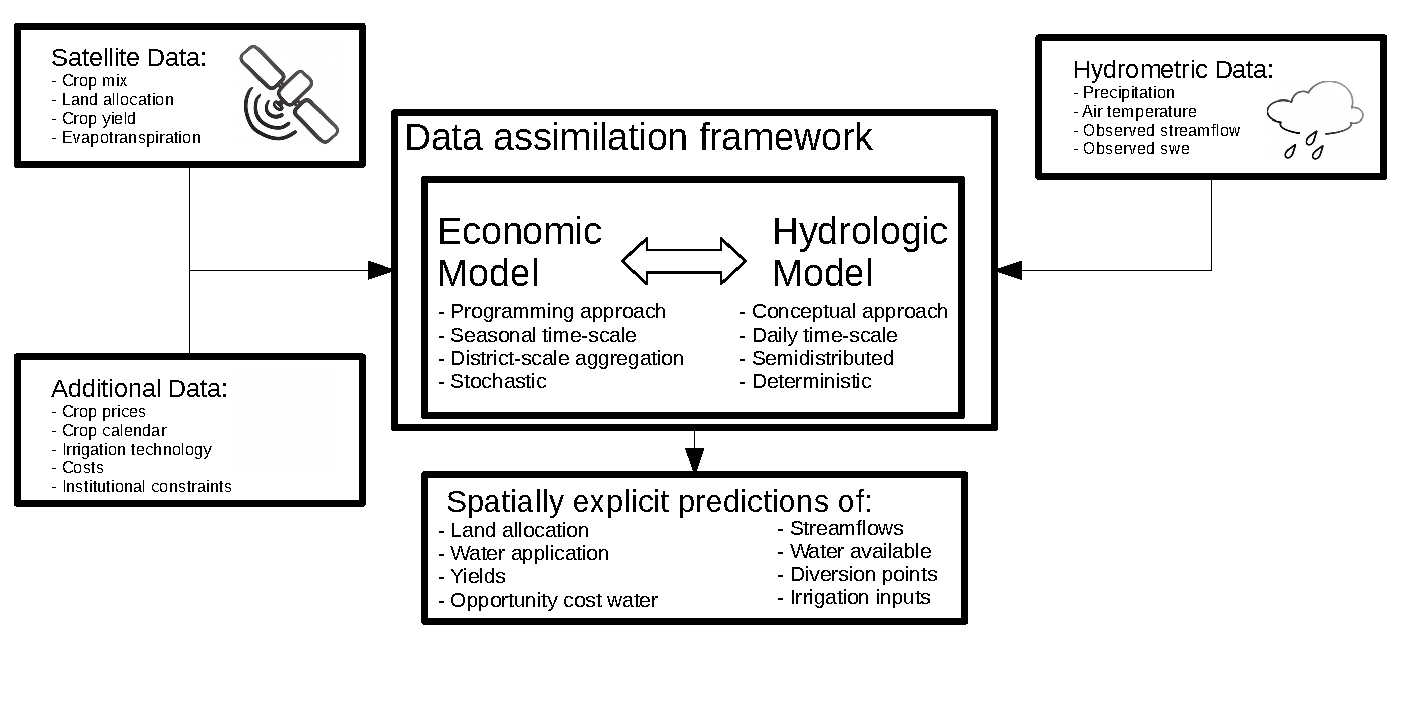
\includegraphics[width=\textwidth]{Figures/DA_approach.pdf}
    \caption{Overview of the hydro-economic modeling package. An economic model of agricultural production is linked to a spatially explicit hydrologic model and embedded in a stochastic data assimilation framework. The data assimilation framework adjusts the economic component parameters based on the ingestion of remote sensing observations of agricultural activity and other hydrometric and ancillary data. Once the model is calibrated, it can be used to predict probabilities of resource allocation under designed climate and policy scenarios.}
    \label{fig:DAFramework}
\end{figure}

\subsection{Economic model of agriculture and farmer behavior}

The backbone of the economic component is a nonlinear constrained optimization model calibrated to capture observed producer behavior using the PMP method \citep{Howitt1995}. The PMP approach is grounded in the assumption that producers allocate resources, in our case land and water, to maximize their net revenues subject to resource constraints:

% \begin{equation}\label{eq:net_revs}
%     \begin{split}
%         \max_{ x_{land,i} , x_{water,i} \geq 0 } net = \quad \sum_i \left{ p_i \pi_i\left( x_{land,i}, x_{water,1}; \mu, \beta_{land,i},\beta_{water,i}, \rho_{i}, \delta_{i} \right) \\- \left( c_{land,i} + \lambda_{land,i} \right) x_{land,i} - \left( c_{water,i} + \lambda_{water,i} \right) x_{water,i} \right} \\
%     \text{subject to} \quad\sum_{i} x_{ i 1 } \leq \overline{L} \left[ \overline{ \lambda }_{ 1 } \right]
%     \end{split}
% \end{equation}

% \begin{multline}\label{eq:net_revs}
%         \max_{ x_{land,i} , x_{water,i} } net = \quad \sum_i \left\{ p_i \pi_i\left( x_{land,i}, x_{water,i}; \mu_i, \beta_{land,i},\beta_{water,i}, \rho_{i}, \delta_{i} \right) -  c_{land,i} x_{land,i} - c_{water,i} x_{water,i} \right\} \\
%     \text{subject to: }\\ \quad\sum_{i} x_{land,i} \leq \overline{L} \left[ \overline{ \lambda }_{fsl} \right]\\
%     x_{land,i} = x_{land,i}^{obs} \left[ { \lambda }_{land,i} \right]\\
%     x_{water,i} = x_{water,i}^{obs} \left[ { \lambda }_{water,i} \right]\\
%     x_{land,i} , x_{water,i} \geq 0\\
% \end{multline}
\begin{multline}\label{eq:net_revs}
        \max_{ x_{land,i} , x_{water,i} } net = \quad \sum_i \left\{ p_i \pi_i\left( x_{land,i}, x_{water,i}; \mu_i, \beta_{land,i},\beta_{water,i}, \rho_{i}, \delta_{i} \right) -  c_{land,i} x_{land,i} - c_{water,i} x_{water,i} \right\} \\
    \text{subject to: }\\ 
    \quad\sum_{i} x_{land,i} \leq \overline{L} \left[ \overline{ \lambda }_{L} \right]\\
    \quad\sum_{i} x_{water,i} \leq \overline{W} \left[ \overline{ \lambda }_{W} \right]\\
    x_{land,i} , x_{water,i} \geq 0\\
\end{multline}

\noindent where $net$ is net revenue, defined as revenue less the costs of land and water use; the index $i = 1,...,I$ represents crops; $x_{land,i}, x_{water,i}$ represent land and water resource inputs for crop $i$, respectively; $p_i$ is the price received for crop $i$; $\pi_i$ is a production function that maps resource inputs to total production of crop $i$; and $c_{land,i}$, $c_{water,i}$ are the unit costs associated with land and water use to produce crop $i$. The parameters $\mu, \beta, \rho, \delta$ are production function parameters to be calibrated using PMP. The constraints in problem (1) state that the total land and water used for all crops in the region must be less than or equal to the total land $\overline{L}$ and water $\overline{W}$ available for cultivation and that resource allocation has to be non-negative. The total land and water available for cultivation may be constrained by physical limits (e.g., streamflow) or by policy or other institutional constraints (e.g., water rights or storage release policies). 

Consistent with the recent economic literature on PMP \citep{Merel2011b}, we define the production function in Eq. \eqref{eq:net_revs} using a generalized constant elasticity of substitution (CES) functional form: 

\begin{align}\label{eq:produc_func}
    \pi_i = \mu_i \left[ \beta_{land,i} x_{land,i} ^ { \rho_i } + \beta_{water,i} (x_{water,i} + x_{precip,i}) ^ {\rho _i} \right]^{ \frac { \delta_i}{ \rho_i} }
\end{align}

A limitation of previous research in this area is that it has differentiated the production function in Eq. \eqref{eq:produc_func} for irrigated and non-irrigated crops, requiring independent calibration of each function \citep[e.g.][]{Maneta2009c}. In this study, we streamline calibration by incorporating a production function that can handle irrigated and non-irrigated cases. To do so, we separate the total amount of water available to support crop growth into an exogenous component provided by natural sources like precipitation $x_{precip,i}$ (not controlled by the farmer), and an endogenous component provided by supplemental irrigation, $x_{water,i}$ (controlled by the farmer). This formulation also allows us to differentiate the costs of providing water for crop production, which differ depending on whether a year has relatively wet or dry conditions. %Therefore, equation \eqref{eq:net_revs} defines $x _ { i 2 } ^ { * } = x _ { 20 } + x _ { i 2 }$, where $x_{20}$ is natural ET and $x_{i2}$ is applied ET (irrigation).

\subsection{Hydrologic component}

The hydrologic component provides water availability constraints to agricultural production. Precipitation is transformed into runoff using a gridded version of the HBV model \citep{Bergstrom1973, Bergstrom1995, Lindstrom1997}. When runoff reaches the channel it is routed through the stream network using the Muskingum-Cunge method \cite{Cunge1969}. Both models are well-known and documented, and because of its parsimonious nature, reliability, robustness, and performance they have been widely applied in many regions of the world for hydrologic response analysis under climate change and drought \citep{Driessen2010, Menzel2002}. 

HBV is a precipitation-runoff model originally developed to assist in flood forecasting in Sweden. The hydrologic system is conceptualized as a cascade of four compartments: snowpack, soil, upper groundwater zone, and lower groundwater zone in each of the hydrologic response units (HRUs) in which the user may divide the region (Appendix \ref{app:hydrologic_model}). Water outputs from the soil and groundwater compartments of each HRU are transformed into runoff by convolution with a triangular unit hydrograph. We implemented this particular application as a partially gridded version of the original model. The model uses gridded (raster) daily precipitation, and maximum and minimum daily air temperature and produces the aggregated (spatially averaged) runoff response of the different subcatchments composing the study area. Water ponded on the surface of pixel $k$ at time $t$ available for infiltration and for the generation of runoff is the integration of water input rates from snowmelt $Melt_{k,t}$, rainfall $Rain_{k,t}$  and supplemental irrigation $P^{irr}_{k(j),t}$ if pixel $k$ is in the set of pixels designated to be irrigated from water source $j$,

\begin{align}
Pond_{k,t} &= Pond_{k,t-1} + (Melt_{k,t} + Rain_{k,t} +  P^{irr}_{k(j),t})\Delta t - \Delta SM_{k,t} 
\end{align} 

Infiltration (described in \ref{app:hydrologic_model}) increases the water storage in the soil ($\Delta SM_{k,t}$) at pixel $k$ and is aggregated over all pixels $k$ within subcatchment $l$. When water stored in the soil moisture compartment of subcatchment $l$ reaches a threshold, the excess water generates output or percolates to the groundwater compartment. Outputs from the soil and groundwater compartments produce the integrated response of the subcatchment. A comprehensive description of our particular implementation of the model is provided in \ref{app:hydrologic_model}. In total, the hydrologic model tracks four internal states in each of the subcatchments: snow water equivalent, soil water storage, water storage in the upper groundwater compartment and water storage in the deep water compartment. The model has \num{12} parameters that can be potentially tuned. Details of the model structure and implementation are provided in \ref{app:hydrologic_model}. 

The runoff response of each subcatchment becomes lateral water contributions into the stream reach contained in the subcatchment. Lateral runoff and inflows from upstream subcatchments are routed through the river network using the Muskingum-Cunge model. The Muskingum model uses a two-parameter constitutive equation to relate storage ($S$) in a reach to its inflows ($Q_{in}$) and outflows ($Q_{in}$): $S = K\left[eQ_{in} + (1 - e)Q_{out}\right]$, where $K$ and $e$ are the two function parameters.  This constitutive relationship permits to write the mass balance equation for the reach as a function of streamflows and parameters. The Muskingum-Cunge method uses this relationship to develop a finite difference approximation of the 1D diffusion equation:

\begin{align}
&Q_j^{t+1}\left[K_j(1 - e_j) + 0.5\Delta t  \right] + Q_{j-1}^{t+1}\left[K_je_j - 0.5\Delta t  \right]  \\
&= Q_j^{t}\left[K_j(1 - e_j) - 0.5\Delta t  \right] + Q_{j-1}^{t}\left[K_je_j + 0.5\Delta t  \right]\\
&+ (q_{j}^{t+1} - q^{irr}_{j,i,t+1}) \left[K_j(1 - e_j) + 0.5\Delta t  \right]
\end{align}

Full details on the Muskingum-Cunge algorithm and its implementation  are provided in \ref{app:hydrologic_model}.


\subsection{Model coupling}

The hydrologic component of the model operates deterministically at daily time steps and at variable spatial resolutions defined by the size of the HRUs. On the other hand, the economic component operates stochastically at seasonal time steps and at spatial resolutions defined by counties, districts, or regions that may or may not be coincident with the HRUs. To couple the two components, relevant information generated by one component needs to be spatially and temporally aggregated or disaggregated to match the resolution of the receiving component. At the beginning of each simulated year, the economic component is run over each economic unit in the domain and the probabilistic ensemble of land $\mathbf{x}_{land, i}$ and water $\mathbf{x}_{water, i}$ allocated to each crop $i$ for the growing season are determined. The average of the ensemble of seasonal water allocations $\mathbb{E}[\mathbf{x}_{water, i}]$ are temporally disaggregated to obtain expected daily diversions from the hydrologic network. Diverted water is then allocated to irrigated fields as supplemental precipitation. The temporal disaggregation of the seasonal irrigation volume to daily water diversion rates is achieved by redistributing the total crop water requirements over the growing season according to the growth stage of the crop as reflected by its crop coefficient:    

\begin{align}
    &q^{irr}_{j,i,t+1} = \frac{  \mathbb{E}[\mathbf{x}_{water, i}]*\omega_{t}}{I_{eff_i}}\\
     \nonumber &\text{where: }\\ 
    &\omega_{i,t+1} = \frac{Kc_{i,t+1}}{\sum_t Kc_{i,t+1}},
\end{align}

\noindent where $q^{irr}_{j,i,t+1}$ is the water diverted for irrigation from river node $j$ for crop $i$ at day $t+1$, $I_{eff_i}$ is an irrigation and conveyance efficiency factor for crop $i$, and $\omega_{i,t+1}$ is a weight factor that reflects the daily fraction of the total crop water requirement according to the crop coefficient $Kc_{i,t+1}$.

Water diverted each day from a given river node is applied as supplemental irrigation over pixels with land use designated as irrigated crop in the corresponding economic unit. Irrigation is applied uniformly over all pixels designed as irrigated crops: 

\begin{align}
    P^{irr}_{k(j),t+1} = \frac{\sum_i q^{irr}_{j,i,t+1} }{N_k, \Delta x^2},
\end{align}

\noindent where $P^{irr}_{k(j),t}$ is the supplemental irrigation applied at time $t$ on pixel $k$ from the set of pixels classified as irrigated agriculture within the economic unit associated with diversion point $j$, $N_k$ is the total number of pixels classified as irrigated agriculture within the economic units, and $\Delta x^2$ is the pixel area. 
